\documentclass{article}
\usepackage{color}
%% The amsthm package provides extended theorem environments
%% \usepackage{amsthm}
%% The amsmath package provides equation environment
\usepackage{amsmath}
\usepackage{graphicx}

% upright sub-index
\newcommand{\ui}[2]{#1 _{\text{#2}}}
% upright sub-index with variable
\newcommand{\uis}[3]{#1 _{\text{#2}, #3}}

\title{List of Changes and Answers to Reviewers}
% \title{}
\author{Adaptable and Interpretable Framework for Anomaly\\Detection in SCADA-based Industrial Systems
  \\M. Wadinger, M. Kvasnica}
\makeatletter
\newenvironment{comment}{
\begin{sloppypar}\slshape
\vspace{5 mm}
\color{blue}
%$\rightarrow$
 \@beginparpenalty\@M
  \begin{list}{}{\setlength{\topsep}{0ex}%
  \setlength{\leftmargin}{\rightmargin}}\item[]
 \@beginparpenalty\@endparpenalty
}
{\end{list}
\end{sloppypar}
%$\leftarrow$
}
\makeatother

\def\RIsatmax{\overline{\mathcal{R}}}
\def\RIsatmin{\underline{\mathcal{R}}}
\def\RIunsat{\mathcal{U}}

\bibliographystyle{alpha}

\begin{document}
\maketitle


\section{List of Changes}

List of main changes:
\begin{enumerate}

  %   \item The manuscript was shortened to $7$ pages.
  %   \item The leading paragraph of Section 4 was reworded to address
  %         reviewers' comments on SVMs.
  %   \item Section 4.1 was removed, linear separation is now tackled as a
  %         special case in the {\em Polynomial Separation} section (labeled as
  %         Section 4.1 in the revision).
  %   \item Big-O notation in Section 5 was replaced by hard figures
  %         indicating required computation and consumed memory.
  %   \item Section 6.2 was enriched to address reviewers' comments.
  %   \item Conclusions was modified according to reviewers' requests.
  \item Introduction was enriched to address reviewers' comments.
  \item Figure 2 was added to illustrate the definition of anomalies to address reviewers' comments.
  \item Captions in Figures 5, 6, 7 (labeled as Figures 4, 5, 6 in the previous manuscript) were reworded to make them more illuminating.
  \item Table 2 was transposed to allow for new metrics to be added.
  \item False Alarm Rate, AUC, and Mean of Rolling AUC were added to the results in Table 2 to address reviewers' comments.
  \item Section 4.4 was added to address reviewers' suggestion on scalability analysis.
\end{enumerate}

\section{Answers to Reviewers and to the Associate Editor}

We would like to thank all reviewers and to the associate editor for
encouraging comments and hints. We have tried to address all of them
appropriately.

\subsection*{Associate Editor}

\begin{comment}
Reviewers have now commented on your paper. You will see that they are advising that you revise your manuscript. If you are prepared to undertake the work required, I would be pleased to reconsider my decision.

For your guidance, reviewers' comments are appended below.

If you decide to revise the work, please submit a list of changes or a rebuttal against each point raised by the reviewers. You can upload this as the 'Detailed Response to Reviewers' when you submit the revised manuscript.
\end{comment}
{\bf Response:}
We would like to thank the associate editor for his/her evaluation. We
believe that the modifications, described in more detail below,
address all issues pointed out by the reviewers.

\subsection*{Reviewer 1}
\begin{comment}
This paper proposes a new online anomlay detection method and verifies its effectiveness on real-world datasets. However, there are some limitations as follows:
\end{comment}

\begin{enumerate}

  \item
        \begin{comment}
        There is no clear definitions of point anomaly, collective anomalies and concept changes. Figure 2 does not illustrate their differences either.
        \end{comment}
        {\bf Response:}
        Thank you for your suggestion. We have added Figure 2 in the revision to illustrate the distinctions between these anomaly types. Figure 2, previously in question, is now labeled as Figure 3 in the revision.

        Figure 2 depicts a sample of each of the three scenarios: point anomaly (measurement with significant dissimilarity), collective anomaly (cluster of abnormal points), and change point (initial sequence of changed operation) detection.

  \item
        \begin{comment}
        The captions of Figures 4,5,6 are similar but the labels are different. It is a bit confused as which one is the ground truth.
        \end{comment}
        {\bf Response:}
        The reviewer is correct that the captions are too similar. We have updated the captions in the revised manuscript to eliminate any confusion. Please note that Figures 4, 5, and 6 in the initial submission are now labeled as Figures 5, 6, and 7 in the revised manuscript due to the addition of Figure 2 to address the reviewer's previous comment.

        The changes made to the captions include a description of two model setups: without adaptation to change points in Figure 5 and with adaptation to change points in Figures 6 and 7. Though an identical model setup is depicted in Figures 6 and 7, Figure 7 shows the accompanying task of sampling anomaly detection in addition. This way, we could better highlight specific features that build up our proposed AID method.

        It is important to note that the challenge of obtaining precise ground truth information remains. Operators did not inform us about the exact time of abnormal events, introducing ambiguity. While we refer to the dates of the events in Section 4.1, selecting the time of the anomaly for plotting purposes would be arbitrary and compromise the objectivity of the results. Therefore, Figures 5, 6, and 7 do not bear information about ground truth.

  \item
        \begin{comment}
        There are other self-supervised change-point detection method, such as ~\cite{Deldari2021}.
        \end{comment}
        {\bf Response:}
        We appreciate the reviewer's suggestion and acknowledgment of the reference ~\cite{Deldari2021}. We have incorporated the reference into the Introduction section of the paper to enrich the discussion.

        We found the suggested reference highly relevant in the paragraph discussing the need for an early change point detection mechanism. After mentioned remark of Tartakovsky from 2013~\cite{Tartakovsky2013}, that the immediate change point detection is not a feasible option unless there is a high tolerance for false alarms, we refer to the contrastive learning approach of reviewer's suggested reference~\cite{Deldari2021} as a promising balance between early transition detection and low false alarm rate. We believe this helps to reflect the current state of the research better.
  \item
        \begin{comment}
        It seems that using ARIMA or moving average can easily detect the anomalies or change points on the real-world datasets.
        \end{comment}
        {\bf Response:}
        We acknowledge this observation of ARIMA and moving averages usage for anomaly and change point detection tasks on real-world datasets. To address this observation, we included in the Introduction two recent publications dealing with offline vectorized adaptation of ARIMA for complex systems. Moreover, the reviewer's suggestion motivated our effort to apply methods from this family to data from the first case study. We were unable to find a suitable implementation of online-trained ARIMA for vectorized usage, resulting in the selection of an online univariate implementation. Due to the univariate nature and limitations discussed below, we did not include the results in the revised manuscript.

        Referring to Figure~\ref{fig:snarimax}, it seems that unique challenges posed by online anomaly detection in evolving data streams within real-world datasets present some obstacles for ARIMA and moving average methods.

        In an effort to achieve the best performance, we performed Bayesian optimization of the Seasonal Non-linear AutoRegressive Integrated Moving-Average with eXogenous inputs model (SNARIMAX)~\cite{Anava2013} and its special parametrization cases for the data from the first case study. Various metrics, with and without running mean, were tested in the cost function, selecting Median Absolute Error (MedAE) as one with the best convergence and highest robustness toward anomalies. Five step ahead forecast of normalized temperature was used for evaluation, showing a good balance between anomaly discrimination and accurate tracking. We made several observations on the performance of the methods.

        \begin{figure}[htbp]
          \centerline{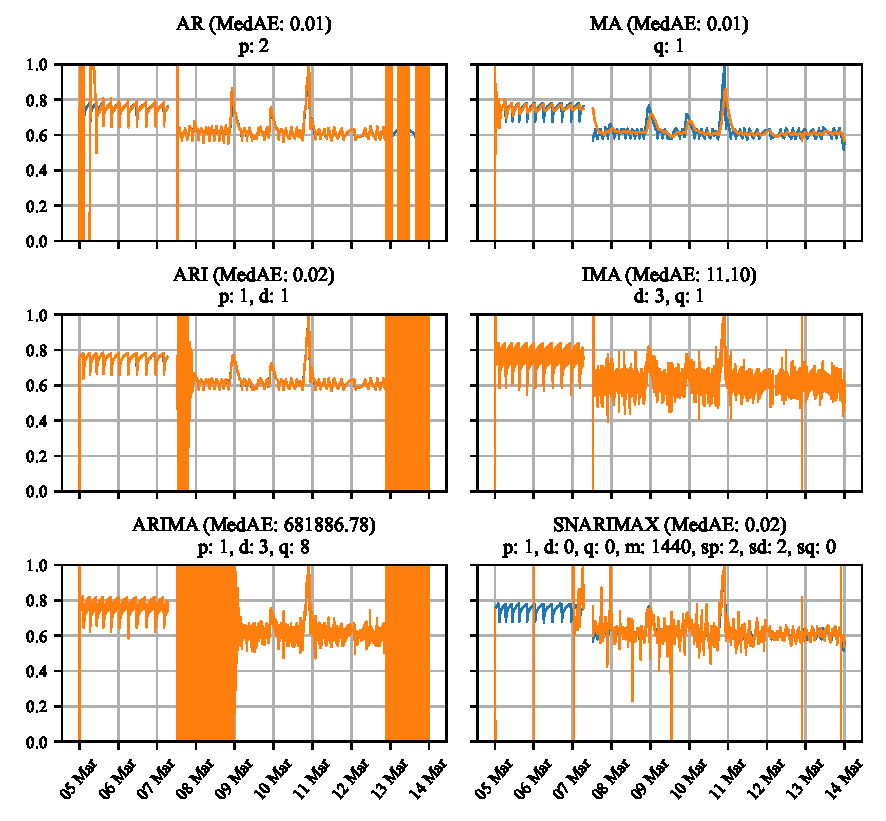
\includegraphics[width=\textwidth]{ARIMA_opt_results.pdf}}
          \caption{Comparison of five-step ahead forecast (orange) of normalized temperature (blue) using various parametrization of SNARIMAX model and special parametrization cases (AR, MA, ARI, IMA, ARIMA) with optimized parameter values. The forecast is aligned with the original data.}
          \label{fig:snarimax}
        \end{figure}

        Firstly, the moving average (MA) method's forecast alone discriminates outliers well. Nevertheless, it shows little sensitivity to abrupt regular changes of temperatures from 5th to 7th March, which would be falsely marked as anomalous, along with true anomalies by a simple threshold filter. Secondly, the autoregressive (AR) method exhibits high sensitivity to point anomaly before 13th March, resulting in ongoing instability (though barely visible, sensor reports 0.0 on 12th March from 21:15 to 21:22 in Figure~\ref{fig:snarimax}).

        Using differencing to remove trends and seasonality with the AR method (ARI) further decreased stability during the formerly mentioned event starting on 12th March at 21:15 and, combined with the moving average method (IMA), added significant noise to predictions during whole evaluated history. Despite hyperparameter optimization and evaluation with engineered time-based features, we did not observe satisfactory results with ARIMA and SNARIMAX models.

        Protection of the model from learning anomalous data through threshold filters, to mitigate their effect on the model's performance, and intelligent adaptation to change points and non-stationary may improve the performance. Nevertheless, due to the extent of the work required, we decided to leave the inclusion of these features as a potential avenue for future work.

        A critical feature of our proposed method within SCADA-based systems is the ability to dynamically render process limits for individual signals, enhancing diagnostic capabilities. While a similar task could be achieved with ARIMA, it requires extensive fine-tuning of an ensemble of ARIMA models for each signal in the system. Vectorization of this task may significantly speed up this process.

        Our literature review indicates that Vector Autoregression, the multivariate extension of ARIMA, could efficiently model multivariate time series, as explored in papers such as \cite{Melnyk2016, Zhang2023}. However, our research focuses on online anomaly detection for evolving data streams, and the need for a vectorized implementation for online-trained ARIMA limits its usage in our comparisons. Future research could explore extending ARIMA to its multivariate counterpart for online training.

        Integrating our proposed method with forecasting models during feature engineering, as demonstrated in Section 4.1 for physics-based model utilization, presents a promising direction for enhancing performance with the aid of the ARIMA method.

  \item
        \begin{comment}
        It would be better to use AUC rather than F1 to measure the anomaly detection performance. Moreover, range-based AUC is even better and more fair for streaming or sliding window-based method.
        \end{comment}
        {\bf Response:}
        We agree with the reviewer that AUC, in general, is a better metric for imbalanced datasets. In response to the reviewer's recommendation, we have included AUC in the results presented in Table 2 of the revised paper. Adding AUC provides an alternative perspective on performance that may interest the reader.

        We tried to implement hyperparameter optimization with AUC. Nevertheless, due to the poor convergence of the reference methods on benchmark data, we decided to use the F1 score, which showed better convergence for all three compared methods.

        Additionally, we were unaware of the range-based AUC metric during paper writing and result collection. After this suggestion, we computed the mean value of range-based AUC using the implementation from~\cite{Brzezinski2017} and enriched the results in Table 2.

        We also attempted to use the mean value of range-based AUC for hyperparameter optimization. Due to minimal improvement in performance compared to regular AUC, we decided to retain the F1 score as the optimized metric. The results obtained using the range-based AUC metric in the hyperparameter optimization cost function are provided in Table~\ref{tab:perf_comp_rollauc} for reference. We highlight that the false positive rate dropped by 10 \% compared to the model optimized on the F1 score. This is a significant improvement in the context of anomaly detection, where false alarms have higher priority than precision or recall.

        We hope these additions to the revised manuscript and explanations in this response enhance the transparency and completeness of our evaluation.

\end{enumerate}


\begin{table}[htbp]
  \caption{Evaluation of models optimized for Rolling AUC score on SKAB dataset. The best-performing model is highlighted in bold. Values in brackets represent macro values of the metric.}
  \begin{center}
    \label{tab:perf_comp_rollauc}
    \begin{tabular}{|l|c|c|c|c|}
      \hline
      \textbf{Algorithm}      & AID                    & HS-Trees          & OC-SVM            \\
      \hline
      Precision [$\%$]        & $\boldsymbol{47}$ (60) & 30 (47)           & 32 (48)           \\
      \hline
      Recall [$\%$]           & $\boldsymbol{55}$ (61) & 4 (50)            & 3 (50)            \\
      \hline
      F1 [$\%$]               & $\boldsymbol{51}$ (60) & 7 (42)            & 6 (42)            \\
      \hline
      AUC [$\%$]              & $\boldsymbol{61}$      & 50                & 50                \\
      \hline
      Mean Rolling AUC [$\%$] & $\boldsymbol{60}$      & 50                & 49                \\
      \hline
      FPR [$\%$]              & 38                     & $\boldsymbol{37}$ & $\boldsymbol{37}$ \\
      \hline
    \end{tabular}
  \end{center}
\end{table}

\subsection*{Reviewer 2}
\begin{comment}
This paper presents an interesting and potentially useful framework called AID for anomaly detection and root cause diagnosis in industrial internet-of-things (IoT) systems. It incorporates dynamic conditional probability distribution modeling to adapt to non-stationary data streams, which is crucial for industrial systems. And industrial case studies demonstrate capabilities on real systems. However, i still have following concerns.
\end{comment}

\begin{enumerate}
  \item
        \begin{comment}
        More analysis of computational complexity and scalability limitations for high-dimensional industrial systems would strengthen the work.
        \end{comment}
        {\bf Response:}
        Thank you for bringing attention to the importance of computational complexity and scalability in the context of high-dimensional industrial systems. To address this suggestion, we have incorporated Section 4.4 into our revised manuscript, providing a dedicated analysis of scalability and time complexity.

        In Section 4.4, we delve into the computational complexities and scalability limitations of our proposed method in the context of high-dimensional industrial systems. The section aims to offer insight into the scalability of the proposed method for anomaly detection tasks and in the context of SCADA-based systems where dynamic limits are of interest. Evaluation is performed on the data from the first case study, enriched with additional signals from other modules in the system, resulting in a total of 60 signals.

        Table~\ref{tab:latency} (Table 4 in the revised manuscript) presents the latency analysis of the proposed method AID with a varying number of features. The results indicate that the latency of the proposed method grows increasingly with the number of features. The minimum latency reflects the time required to process a single sample during the grace period, while maximum latency reflects the time required when multiple samples are processed at once.

        \begin{table}[htbp]
            \caption{Latency analysis of the proposed method AID with varying number of features.}
            \begin{center}
                \label{tab:latency}
                \begin{tabular}{|l|c|c|}
                    \hline
                    \begin{tabular}[c]{@{}l@{}}\textbf{Number of}\\ \textbf{Features}\end{tabular} & \begin{tabular}[c]{@{}c@{}}\textbf{Detection}\\$\mu \pm \sigma$ ($\min$, $\max$) [ms]\end{tabular} & \begin{tabular}[c]{@{}c@{}}\textbf{Detection + Limits}\\$\mu \pm \sigma$ ($\min$, $\max$) [ms]\end{tabular} \\
                    \hline
                    1 & $0.37 \pm 0.26~(0.05, 31.7)$ & $0.63 \pm 0.38~(0.23, 35.9)$ \\
                    10 & $2.25 \pm 0.92~(0.10, 13.6)$ & $5.24 \pm 0.98~(0.80, 15.1)$ \\
                    20 & $5.46 \pm 2.16~(0.26, 30.6)$ & $14.7 \pm 2.27~(1.10, 47.5)$ \\
                    30 & $10.9 \pm 4.31~(0.52, 42.4)$ & $34.3 \pm 4.50~(2.59, 72.4)$ \\
                    40 & $20.7 \pm 8.15~(0.89, 52.7)$ & $69.5 \pm 8.57~(2.84, 140)$ \\
                    50 & $97.3 \pm 47.4~(1.36, 1010)$ & $297 \pm 59.4~(3.94, 1330)$ \\
                    60 & $142 \pm 71.2~(1.95, 1640)$ & $468 \pm 111~(7.08, 3710)$ \\
                    \hline
                \end{tabular}
            \end{center}
        \end{table}

        Figure~\ref{fig:latency} showing the distributions of the latency for a varying number of features indicate that the mean latency is cubic in the number of features in the detection task while inclines to quartic in the combined task of detection and dynamic operating limits setting.

        \begin{figure}
          \centering
          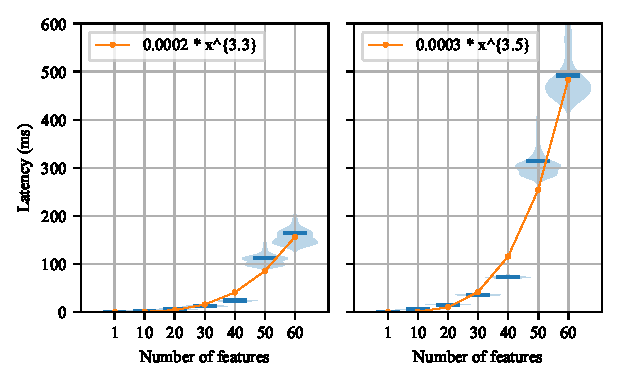
\includegraphics[width=\textwidth]{scalability.pdf}
          \caption{Analysis of latency distribution of the proposed method AID. Violin plots depict the distribution of the latency for varying number of features, while horizontal bars show mean latency.}
          \label{fig:latency}
        \end{figure}

        We hope that this addition will enhance the completeness of our work.

  \item
        \begin{comment}
        While the paper mentions comparisons with other methods, it lacks detailed benchmarking data, such as false positive rates.
        \end{comment}
        {\bf Response:}
        We appreciate the reviewer's insightful comment regarding the need for more detailed benchmarking data, particularly including false positive rates. In response, we have added a False Positive Rate (FPR) to the results in Table 2 of the revised manuscript (Table~\ref{tab:perf_comp_f1} in this document), addressing this specific concern.

        Additionally, to provide a more comprehensive view of the model's performance on imbalanced datasets while addressing other reviewers' comments, we have included AUC and mean of range-based AUC in Table 2 of the revised manuscript. These metrics offer further insights into the detection capabilities of our proposed method. In Table~\ref{tab:perf_comp_f1} we observe that our proposed AID method outperforms the reference methods in terms of added metrics on the benchmark dataset.

        \begin{table}[htbp]
          \caption{Evaluation of models optimized for F1 score on SKAB dataset. The best-performing model is highlighted in bold. Values in brackets represent macro values of the metric.}
          \begin{center}
            \label{tab:perf_comp_f1}
            \begin{tabular}{|l|c|c|c|c|}
              \hline
              \textbf{Algorithm}      & AID                    & HS-Trees            & OC-SVM              \\
              \hline
              Precision [$\%$]        & $\boldsymbol{41}$ (59) & 36 (51)             & 39 (54)             \\
              \hline
              Recall [$\%$]           & $\boldsymbol{80}$ (59) & 74 (51)             & 63 (54)             \\
              \hline
              F1 [$\%$]               & $\boldsymbol{54}$ (53) & 48 (44)             & 48 (52)             \\
              \hline
              AUC [$\%$]              & $\boldsymbol{59}$      & 51                  & 54                  \\
              \hline
              Mean Rolling AUC [$\%$] & $\boldsymbol{57}$      & 50                  & 53                  \\
              \hline
              FPR [$\%$]              & $\boldsymbol{47}$      & 56                  & 48                  \\
              \hline
              Avg. Latency [ms]       & 1.45                   & $\boldsymbol{0.05}$ & $\boldsymbol{0.05}$ \\
              \hline
            \end{tabular}
          \end{center}
        \end{table}

  \item
        \begin{comment}
        Comparing diagnosis accuracy for root causes against other interpretable methods could better highlight capabilities.
        \end{comment}
        {\bf Response:}
        % Prejav v clanku
        We appreciate the reviewer's suggestion regarding the comparison of diagnosis accuracy for root causes against other interpretable methods. We recognize the importance of addressing this aspect, resulting in a comparison with the diagnostic method DBStream. We have tried hard to convey the results of this comparison in a clear and concise manner in the paper. However, we could not manage without significantly extending the page range, which we found inappropriate at this stage of writing the paper.

        As we have recognized the challenges of adapting analogous interpretable methods from cited publications in our paper~\cite{Yang2022, Steenwinckel2021} due to undisclosed or non-adaptable code, we decided to compare our proposed method with DBStream~\cite{Hahsler2016}, an online version of DBScan designed for evolving data streams.

        It is an unsupervised method with the ability to disregard anomalies and capture clusters of various sizes and densities. It has been successfully used throughout the literature for diagnostic purposes. In~\cite{Li2019}, DBScan was used for thermal runaway diagnosis of battery systems in electric vehicles, relying on engineered features reflecting battery performance. Other applications include power transformer fault diagnosis~\cite{Liu2020} and fault diagnosis of rolling bearing~\cite{Li2020}.
        Its usage in these applications, with expert knowledge of the system, involves mapping clusters to root causes, making it a promising method for our comparison.

        The comparison was performed on the Controlled Anomalies Time Series (CATS) Dataset, a simulated complex dynamical system with 200 injected anomalies. This dataset is publicly available and suitable for root cause analysis, as disclosed in the dataset's description. We performed two types of comparisons.

        Firstly, we assessed clustering performance, a key feature of DBStream. This analysis demonstrated the overlap of clusters and various groups of root causes in data. Both methods were optimized to maximize the adjusted mutual information score, a metric that showed the highest importance on synthetic root cause data. The results of this comparison are presented in Table 2.

        Secondly, we compared the ability to detect root causes. Since DBStream does not inherently provide information about root causes, we introduced expert knowledge a posteriori by mapping clusters to ground truth root causes based on the highest overlap. While this approach is artificial, it facilitated a comparison of the methods in root cause detection, with a slight benefit given to DBStream.

        It is important to note that the cluster-to-root cause mapping was also performed while optimizing DBStream's hyperparameters, resulting in a slightly unfair comparison of our proposed method.

        The detailed analysis revealed that our proposed method exhibits a higher weighted precision and better performance regarding macro metrics in root causes detection compared to DBStream. Meanwhile, DBStream exhibits recognizingly higher weighted recall. We have disclosed the results of this comparison in Table 3.

        \begin{table}[htbp]
          \caption{Evaluation of AID and DBStream models optimized for adjusted mutual information score on CATS dataset. The best-performing model is highlighted in bold. Perfect clustering achieves 100\% in each metric.}
          \begin{center}
            \label{tab:perf_comp_cluster}
            \begin{tabular}{|l|c|c|}
              \hline
              \textbf{Algorithm}          & AID               & DBStream \\
              \hline
              Adjusted Mutual Info [$\%$] & $\boldsymbol{13}$ & 2        \\
              \hline
              Adjusted Rand [$\%$]        & $\boldsymbol{20}$ & 1        \\
              \hline
              Completeness [$\%$]         & $\boldsymbol{9}$  & 1        \\
              \hline
              Fowlkes-Mallows [$\%$]      & $\boldsymbol{87}$ & 67       \\
              \hline
              VBeta [$\%$]                & $\boldsymbol{14}$ & 2        \\
              \hline
            \end{tabular}
          \end{center}
        \end{table}


        \begin{table}[htbp]
          \centering
          \caption{Found optimal hyperparameters and searched ranges of AID and DBStream models optimized for adjusted mutual information score on CATS dataset.}
          \label{tab:hyperparam_comp_cluster}
          \begin{tabular}{|l|l|c|c|}
            \hline
            \textbf{Algorithm} & \textbf{Hyperparameters} & \textbf{Found} & \textbf{Ranges} \\
            \hline
            AID &
            \begin{tabular}[c]{@{}l@{}}Threshold\\$\ui{t}{e}$\\$\ui{t}{a}$\\$\ui{t}{g}$\end{tabular} &
            \begin{tabular}[c]{@{}c@{}}0.99973\\22035\\3844\\16667\end{tabular} &
            \begin{tabular}[c]{@{}c@{}}(0.95, 0.99994)\\(150, 30000)\\(50, 10000)\\16667\end{tabular} \\
            \hline
            DBStream &
            \begin{tabular}[c]{@{}l@{}}Cleanup Interval\\Clustering Threshold\\Fading Factor\\Interstection Factor\\Minimum Weight\end{tabular} &
            \begin{tabular}[c]{@{}c@{}}691\\15.68\\0.3547\\1.37\\4.4\end{tabular} &
            \begin{tabular}[c]{@{}c@{}}(1, 1000)\\(0.01, 100)\\(0.0001, 1.0)\\(0.03, 3.0)\\(0.1, 10)\end{tabular} \\
            \hline
          \end{tabular}
        \end{table}

        \begin{table}[htbp]
          \caption{Evaluation of AID and DBStream models optimized for macro of F1 score on CATS dataset. The best-performing model is highlighted in bold. Perfect clustering achieves 100\% in each metric. Values in brackets represent macro values of the metric.}
          \begin{center}
            \label{tab:perf_comp_multiclass}
            \begin{tabular}{|l|c|c|}
              \hline
              \textbf{Algorithm}        & AID                                 & DBStream               \\
              \hline
              Weighted Precision [$\%$] & $\boldsymbol{96}~(\boldsymbol{46})$ & 93~(27)                \\
              \hline
              Weighted Recall [$\%$]    & $86~(\boldsymbol{21})$              & $\boldsymbol{96}~(16)$ \\
              \hline
              Weighted F1 [$\%$]        & $90~(\boldsymbol{26})$              & $\boldsymbol{95}~(18)$ \\
              \hline
              FPR [$\%$]                & $\boldsymbol{1}$                    & $\boldsymbol{1}$       \\
              \hline
            \end{tabular}
          \end{center}
        \end{table}

        \begin{table}[htbp]
          \centering
          \caption{Found optimal hyperparameters and searched ranges of AID and DBStream models optimized for macro of F1 score on CATS dataset.}
          \label{tab:hyperparam_comp_multiclass}
          \begin{tabular}{|l|l|c|c|}
            \hline
            \textbf{Algorithm} & \textbf{Hyperparameters} & \textbf{Found} & \textbf{Ranges}\\
            \hline
            AID &
            \begin{tabular}[c]{@{}l@{}}Threshold\\$\ui{t}{e}$\\$\ui{t}{a}$\\$\ui{t}{g}$\end{tabular} &
            \begin{tabular}[c]{@{}c@{}}0.99981\\20699\\6130\\16667\end{tabular} &
            \begin{tabular}[c]{@{}c@{}}(0.95, 0.99994)\\(150, 30000)\\(50, 10000)\\16667\end{tabular} \\
            \hline
            DBStream &
            \begin{tabular}[c]{@{}l@{}}Cleanup Interval\\Clustering Threshold\\Fading Factor\\Interstection Factor\\Minimum Weight\end{tabular} &
            \begin{tabular}[c]{@{}c@{}}605\\9.25\\0.8090\\0.45\\3.7\end{tabular} &
            \begin{tabular}[c]{@{}c@{}}(1, 1000)\\(0.01, 100)\\(0.0001, 1.0)\\(0.03, 3.0)\\(0.1, 10)\end{tabular} \\
            \hline
          \end{tabular}
        \end{table}

\end{enumerate}

\bibliography{revision}

\end{document}
